% FILE: main.tex  Version 2.1
% AUTHOR:
% Universit�t Duisburg-Essen, Standort Duisburg
% AG Prof. Dr. G�nter T�rner
% Verena Gondek, Andy Braune, Henning Kerstan
% Fachbereich Mathematik
% Lotharstr. 65., 47057 Duisburg
% entstanden im Rahmen des DFG-Projektes DissOnlineTutor
% in Zusammenarbeit mit der
% Humboldt-Universitaet zu Berlin
% AG Elektronisches Publizieren
% Joanna Rycko
% und der
% DNB - Deutsche Nationalbibliothek

\chapter{Discourse-Aware Sentiment Analysis}

Although coarse-grained sentiment analysis methods do a fairly good
job at classifying the overall polarity of a message, putting their
best leg forward to incorporate the compositional principle into that
prediction, a crucial limitation of all these systems is that they
absolutely overlook the structural nature of their input by either
considering it as a single whole (\eg{} bag-of-features approaches) or
analyzing it as a monotone sequence of equally important elements
(\eg{} recurrent neural methods).  Unfortunately, both of these
solutions completely ignore the hierarchical principle of language
\cite{Saussure:90,Hjelmslev:70} which states that complex linguistic
units emerge from the bottom up, by putting together successively
bigger language elements: \eg{} morphemes are united together into
words, several words are joined together into sentences, and multiple
sentences eventually constitue a discourse.  Furthermore, besides this
inherent structural heterogeneity, even units of the same linguistic
level might play a different role and be of unequal importance to the
meaning of the higher-level whole: for example, in words, the root
morpheme typically conveys more lexical information than affixes; in
sentences, the syntactic head normally dominates its grammatic
dependents; and a similar kind of imbalance can also be observed in
discourse, where one of the sentences frequently expresses the gist of
the whole text.

Exactly the lack of discourse information was one of the main reasons
for the misclassifications of the systems of \citet{Severyn:15},
\citet{Baziotis:17}, and our own LBA method shown in Examples
\ref{snt:cgsa:exmp:severyn-error}, \ref{snt:cgsa:exmp:baziotis-error},
and \ref{snt:cgsa:exmp:lba-error}.  Since none of these approaches
explicitly took the discourse structure into account (in the best
case, the inference simply proceeded from the level of words directly
to the level of message), we decided to check whether making the last
of these solutions (the LBA classifier) aware of discourse phenomena
would improve its results.  However, before we present our findings,
we first would like to take a short digression and give an overview of
the most popular approaches to discourse analysis that exist in the
literature nowadays.  Afterwards, in Section~\ref{sec:dasa:data}, we
will describe the way how we inferred and added discourse information
to the PotTS and SB10k data.  Then, in Section~\ref{sec:dasa:methods},
we will summarize the current state of the art in discourse-aware
sentiment analysis (DASA) and also present several own methods,
evaluating their results on the aforementioned corpora.  After
analyzing the effects of different common factors (such as various
subsets of discourse relations and the quality of the downstream
sentiment classification), we will recap our results and draw
conclusions in the last section of this chapter.

\section{Discourse Analysis}\label{sec:dasa:theory}

Since the main focus of this part will be on \emph{discourse
  analysis}, we should first clarify what discourse analysis actually
means and which common ways there are to represent and analyze
discourse automatically.

In a nutshell, discourse analysis is an area of research which
explores and analyzes language phenomena beyond the sentence level
\cite{Stede:11}.  Although the scope of this research can be quite
large (ranging from the use of pronouns in a sentence to the logical
composition of the whole document), in our experiments we will
primarily concentrate on the coherence structure of the text, \ie{}
its segmentation into \emph{elementary discourse units} (EDUs) and
induction of (hierarchical) \emph{coherence relations} between these
EDUs.

Although the idea of splitting the discourse into smaller meaningful
pieces and inferring semantic links between these parts is anything
but new and dates back to the very origins of general linguistics
\cite{Aristotle:10} and in particular its structuralism branch
\cite{Saussure:90}, an especially big surge of interest in this field
happened in the 1970-s with the fundamental works of
\citet{vanDijk:72} and \citet{vanDijk:83}.  In their study of
different stategies of discourse comprehension, the authors introduced
the notion of local and global coherence, defining the former as a set
of ``rules and conditions for the well-formed concatenation of pairs
of sentences in a linearly ordered sequence'' and specifying the
latter as contraints on the macro-structure of the narrative
\cite[see][]{Hoey:83}.  Similar ideas were also proposed
by~\citet{Longacre:79,Longacre:96}, who considered the paragraph as a
unit of tagmemic grammar which was composed of multiple sentences
according to a predefined set of compositional principles.  Almost
contemporarily with these works, \citet{Winter:77} presented an
extensive study of various lexical means which could connect two
sentences and divided these means into two major categories:
\textsc{Matching} and \textsc{Logical Sequence}, depending on whether
they introduced sentences that were rather elaborating on the previous
content or adding new information to the preceding context.

The increased interest of traditional linguistics in text-level
analysis has rapidly spurred the attention of the NLP community to
discourse phenomena.  Among the first who stressed the importance of
discourse structure for automatic generation and understanding of
texts was \citet{Hobbs:79}, who argued that semantic links between
sentences were one the most important component for building a
coherent text.  Similarly to \citeauthor{Winter:77},
\citeauthor{Hobbs:79} also proposed a set of possible inter-sentence
relations which comprised \textsc{Elaboration}, \textsc{Parallel}, and
\textsc{Contrast}.  Although this taxonomy was obviously too small to
accommodate the whole variety of different semantic ties that could
exist between two sentences, this division had laid the foundations
for many successful approaches to automatic discourse processing that
appeared later on.

\textbf{RST} One of the best-known such approaches---\emph{Rhetorical
  Structure Theory} or \emph{RST}---was presented by~\citet{Mann:88}.
Besides revising \citeauthor{Hobbs:79}' inventory of possible
discourse relations and expanding it to a set of 23 elements
(including new items such as \textsc{Evidence}, \textsc{Antithesis},
\textsc{Elaboration}, \textsc{Circumstance}, etc.), the authors also
introduced the distinction between nucleus-satellite (hypotactic) and
multinuclear (paratactic) links, depending on whether the arguments of
these relations were of different or equal importance to the content
of the whole text.  Based on this distinction, they formally described
each relation as a set of constraints on the \emph{Nucleus} (N),
\emph{Satellite} (S), \emph{the N+S combination}, and \emph{the
  effect} of the whole combination on the reader (R).  An excerpt from
the original description of the \textsc{Antithesis} link is shown in
Example~\ref{dasa:exmp:rst-evidence}

\begin{example}[Definition of the \textsc{Antithesis} Relation]\label{dasa:exmp:rst-evidence}
\textbf{Relation Name:} \textsc{Antithesis}

\textbf{Constraints on N:} W has positive regard for the situation
presented in N

\textbf{Constraints on S:} None

\textbf{Constraints on the N+S Combination:} the situations presented
in N and S are in contrast (\ie{} are
\begin{inparaenum}[(a)]
  \item comprehended as the same in many respects,
  \item comprehended as differing in a few respects and
  \item compared with respect to one or more of these differences
\end{inparaenum}
  ); because of an incompatibility that arises from the contrast, one
cannot have positive regard for both the situations presented in N and
S; comprehending S and the incompatibility between the situations
presented in N and S increases R's positive regard for the situation
presented in N

\textbf{Effect:} R's positive regard for N is increased

\textbf{Locus of the Effect:} N
\end{example}

\noindent Using these relations, \citeauthor{Mann:88} then defined the
general structure of a discourse as a projective (constituency) tree
whose nodes were either elementary discourse units or subtrees, which
were connected to each other via semantic edges (relations).

You can see an example of such tree from the Rhetorical Structure
Treebank \cite{Carlson:01a} in Figure~\ref{dasa:fig:rst-tree}.

\begin{figure*}[htbp!]
  {
  \centering
  \dirrel{}{
    \dirrel{Attribution}
           {\rstsegment{\refr{1}}}
           {}
           {\rstsegment{\refr{2}}}}
         {Interpretation-S}
         {\dirrel{Antithesis}
           {\rstsegment{\refr{3}}}
           {}
           {
             \dirrel{Attribution}
                    {\rstsegment{\refr{4}}}
                    {}
                    {
                      \dirrel{}
                             {
                               \dirrel{}{\rstsegment{\refr{5}}}{Comparison}{\rstsegment{\refr{6}}}
                             }
                             {Condition}
                             {\rstsegment{\refr{7}}}
                    }
           }
         }

         \begin{flushleft}
           \begin{rhetoricaltext}
             \unit[1]{Analysts said,}
             \unit[2]{profit for the dozen or so big drug makers, as a group, is estimated to have climbed between 11\% and 14\%.}
             \unit[3]{While that's not spectacular,}
             \unit[4]{Neil Sweig, an analyst with Prudential Bache, said}
             \unit[5]{that the rate of growth will ``look especially good}
             \unit[6]{as compared to other companies}
             \unit[7]{if the economy turns downward.''}
             \rstsource{\cite[WSJ-2341; ][]{Carlson:01a}}
           \end{rhetoricaltext}
         \end{flushleft}
         \caption[RST Tree Example]{Example of an RST-Tree}\label{dasa:fig:rst-tree}
}

\end{figure*}

Despite its immense popularity and practical utility \cite[see
][]{Marcu:98,Yoshida:14,Bhatia:15,Goyal:16}, RST has been often
criticized for the rigidness of the imposed tree constraint
\cite{Wolf:05} and arbitrariness of distinguished relations
\cite{Nicholas:94,Miltsakaki:04}.  As a result of this criticism, two
alternative approaches to automatic discourse analysis have been
proposed in the literature.

\textbf{PDTB} One of these approaches---PDTB (named so after the Penn
Discourse Treebank \cite{Prasad:04})---was developed by the research
group of the University of Pennsylvania
\cite{Miltsakaki:04,Miltsakaki:04a,Prasad:08} and in essence
represents an \emph{underspecification of RST}, where, instead of
fully specifying the hierarchical text structure and providing a
comprehensive set of discourse relations, the authors mainly focused
on the grammatical and lexical means (connectives) which could connect
two sentences.  Typical such means were coordinating or subordinating
conjunctions (\eg{} \emph{and}, \emph{because}, \emph{since}, etc.)
and discourse adverbials (\eg{} \emph{however}, \emph{otherwise},
\emph{as a result}, etc.).  According to the authors' definition, each
such connective had to accept two sentential arguments (\textsc{Arg1}
and \textsc{Arg2}) and express a semantic relationship (\emph{sense})
holding between these predicates.%% The choice
%% of these senses was explicitly restricted for each word: for
%% example, the set of possible senses for \emph{nonetheless} included
%% \textsc{Comparison}, \textsc{Conjunction},
%% \textsc{Contra-Expectation}, and \textsc{Contrast}.

Apart from \emph{explicitly} mentioned connectives, \citet{Prasad:04}
also allowed for situations where these elements were missing from the
text but could be easily inferred by the reader.  They denoted these
cases as \emph{implicit} relations and asked the annotators to label
the arguments of such structures as well, additionally, specifying the
connective which, in their opinion, was omitted.

Finally, if there was no connective at all, \citet{Prasad:04}
distinguished three different possibilities: the coherence relation
\begin{inparaenum}[(i)]
  \item was either expressed by an alternative lexical means which
    made the connective redundant (\textsc{AltLex}), or
  \item it was achieved by referring to the same entities in both
    arguments (\textsc{EntRel}), or
  \item there was no coherence relation (\textsc{NoRel});
\end{inparaenum}
and asked the experts to annotate these situations respectively with
different tags.  Furthermore, in case of reported speech, they also
instructed the annotators to mark the authors of the statements with a
special \textsc{Attribution} label.

Example~\ref{dasa:exmp:pdtb-analysis} shows the previous fragment of
the WSJ corpus now annotated according to the PDTB scheme.  As we can
see from the analysis, the PDTB approach is indeed more flexible in
comparison with RST as it allows discourse units (arguments) to
overlap, be disjoint or even embedded into other segments.  The
assignment of sense relations is also more straightforward and mainly
determined by the connective that links the arguments (\eg{} \emph{in
  fact}, \emph{while}, or \emph{if}).  But, at the same time, the
structure of this annotation is completely flat so that we can neither
infer which of the sentences plays the central role nor see the
modification scope of supplementary statements.

\begin{example}[Example of PDTB Analysis]\label{dasa:exmp:pdtb-analysis}
\fbox{Analysts said,} \argone[1]{profit for the dozen or so big drug
  makers, as a group, is estimated to have climbed between 11\% and
  14\%.}  \connective[1]{\textsc{implicit}$:=$in fact}
\argtwo[1]{\connective[2]{\textsc{explicit}$:=$While}
  \argtwo[2]{that's not spectacular}}, \fbox{Neil Sweig, an analyst
  with Prudential Bache, said} \argtwo[1]{\argone[2]{\argone[3]{that
      the rate of growth will ``look especially good as compared to
      other companies} \connective[3]{\textsc{explicit}:
      if}\argtwo[3]{the economy turns downward}}}.''
\end{example}

\textbf{SDRT} Another alternarive to RST---Segmented Discourse
Representation Theory or SDRT---was proposed by \citet{Lascarides:01}.
Although developed from a completely different angle of view (the
authors of SDRT mainly drew their inspiration from predicate logics,
dynamic semantics, and anaphora theory), SDRT shares many of its
features with the standard rhetorical structure as it also assumes a
graph-like structure of the text, whose nodes are either elementary or
complex discourse units, and distinguishes between coordinating and
subordinating relations.  However, unlike RST, segmented discourse
representation explictly allows the text structure to be any graph and
not only a tree (\ie{} a discourse node can have multiple parents and
also be connected via multiple links to the same vertex), provided
that it does not have crossing dependencies (the right-frontier
constraint).  In this respect, SDRT can be viewed as a
\emph{structural relaxation of RST}.

We can also notice the relatedness of the two approaches by looking at
the SDRT analysis of the WSJ fragment in
Example~\ref{dasa:fig:sdrt-graph}.  Although the names of the
relations in the presented graph differ from those used in RST, many
of these links have the same (or at least similar) meaning as the
respective edges in the first analysis: for example, the
\textsc{Source} relation in SDRT almost completely corresponds to the
\textsc{Attribution} edge in RST, and the \textsc{Contrast} link is
similar to the RST's \textsc{Comparison}.
%% These discrepancies between paratactic dependencies in SDRT and
%% their hypotactic equivalents in RST account for the lion's share of
%% the differences between the two discourse representations in
%% Figures~\ref{dasa:fig:rst-tree} and \ref{dasa:fig:sdrt-graph}.
%% Another dissimilarity stems from the different scopes of the
%% commentary \texttt{While that's not spectacular} assigned by SDRT and
%% RST: while the SDRT graph suggests that this opinion primarily relates
%% to the actual statement of Neil Sweig, RST tree widens the
%% modification scope of this opinion also to the fact of making this
%% statement.

\begin{figure}[htbp]
  \begin{center}
    \begin{tikzpicture}[>=triangle 45,semithick]
      \tikzstyle{edu}=[]; \tikzstyle{cdu}=[draw,shape=rectangle];
      \node[edu] (1a) at (1,0) {$\pi_{1a}$}; \node[edu] (1b) at (1,-2)
           {$\pi_{1b}$};

      \node[edu] (p'') at (7,0)  {$\pi''$};
      \node[edu] (p') at (5.5,-2)  {$\pi'$};
      \node[edu] (1g) at (8.5,-2)  {$\pi_{1g}$};

      \node[edu] (1e) at (4,-4)  {$\pi_{1e}$};
      \node[edu] (1f) at (7,-4)  {$\pi_{1f}$};

      \node[edu] (1c) at (2,-2)  {$\pi_{1c}$};
      \node[edu] (1d) at (4,-2)  {$\pi_{1d}$};

      \draw[->] (1a)  to node [auto] {Source} (1b);
      \draw[->] (1a)  to node [auto] {Narration} (p'');
      \draw[-]  (p'') to node [auto] {} (p');
      \draw[-]  (p'') to node [auto] {} (1g);
      \draw[->] (p')  to node [auto] {Precondition} (1g);
      \draw[-]  (p')  to node [auto] {} (1e);
      \draw[-]  (p')  to node [auto] {} (1f);
      \draw[->] (1e)  to node [auto] {Contrast} (1f);
      \draw[->] (p'') to node [xshift=-8mm,yshift=-0.35mm] {Commentary} (1c);
      \draw[->] (p'') to node [xshift=-0mm,yshift=0mm] {Source} (1d);
    \end{tikzpicture}
    \caption[SDRT graph example]{Example of an SDRT graph}
    \label{dasa:fig:sdrt-graph}
  \end{center}
\end{figure}

\textbf{Final choice} Because it was unclear which of the above
approaches (RST, PDTB, or SDRT) would be more amenable to our
sentiment experiments, we made our decision by taking the following
theoretical and practical concerns into account: From theoretical
perspective, we wanted to have a strictly hierarchical discourse
structure for the analyzed tweets so that we could infer the polarity
of the whole message by recursively accumulating the polarity scores
from less up to more important discourse elements.  From practical
aspect, since there was no discourse parser readily available for
German, we wanted to have a maximal assortment of such parsers for
English so that we could pick one that would be easiest to retrain on
German.  Fortunately, both of these concerns have lead us to the same
solution---Rhetorical Structure Theory, which, on the one hand, was
the only formalism that explicitly guaranteed a single root for the
analyzed text, and, on the other hand, also provided a wide variety of
open-source parsing systems at our disposal
\cite[\eg][]{Hernault:10,Feng:14,Ji:14,Yoshida:14,Joty:15}.

\section{Data Preparation}\label{sec:dasa:data}

To prepare the data for our experiments, we split all microblogs from
the PotTS and SB10k corpora into elementary discourse units using the
ML-based discourse segmenter of~\citet{Sidarenka:15}.  After filtering
out all tweets which had at most one segment,\footnote{Since the focus
  of this chapter is mainly on discourse phenomena, we skip all
  messages which consist of a single discourse segment as their
  overall polarity is unaffected by the discourse structure and can be
  normally determined with the standard disource-unaware sentiment
  techniques.} we assigned polarity scores to the remaining EDUs
(analyzing each of them in isolation) with the help of the
lexicon-based attention classifier.  This left us with a total of
4,771 microblogs (12,137 segments) for PotTS and 3,763 messages (9,625
segments) for the SB10k corpus.  We again used the same 70\%-10\%-20\%
split into training, development, and test sets as we did in our
previous work on coarse-grained sentiment analysis.

%% This figure was generated using the iPython notebook
%% `notebooks/dasa.ipynb`.
\begin{figure*}
  \centering
  {
    \centering
    \begin{subfigure}{0.7\textwidth}
      \centering
      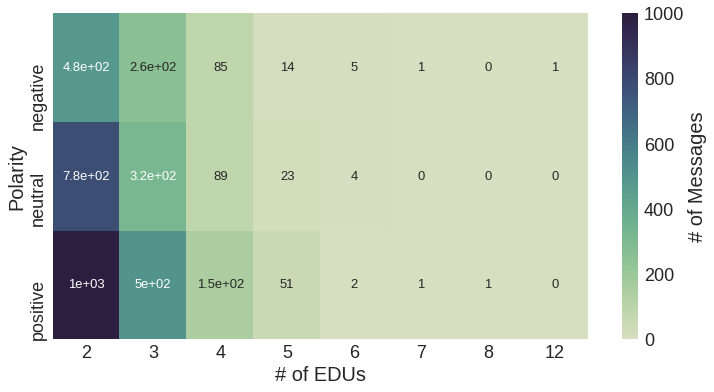
\includegraphics[width=\linewidth]{img/dasa_potts_edu_distribution.png}
      \caption{PotTS}\label{dasa:fig:data-distribution-potts}
    \end{subfigure}
  }
  \centering
  {
    \centering
    \begin{subfigure}{0.7\textwidth}
      \centering
      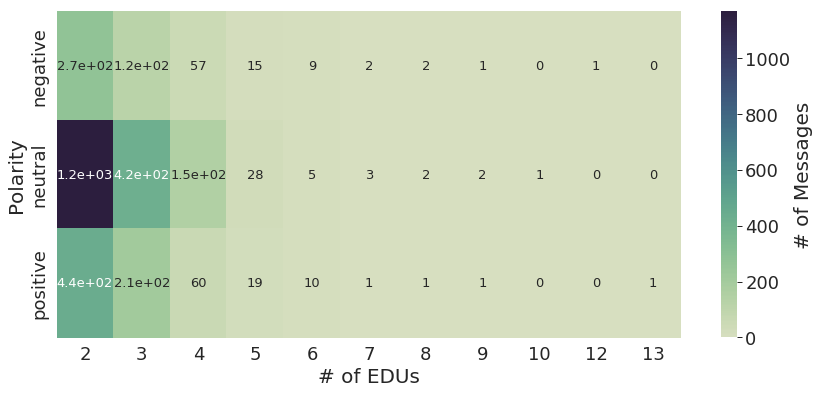
\includegraphics[width=\linewidth]{img/dasa_sb10k_edu_distribution.png}
      \caption{SB10k}\label{dasa:fig:data-distribution-sb10k}
    \end{subfigure}
  }
  \caption[EDU distribution in PotTS and SB10k]{Distribution of
    Elementary Discourse Units and Polarity Classes in the Training and
    Development Sets of PotTS and
    SB10k}\label{dasa:fig:data-distribution}
\end{figure*}

Figure~\ref{dasa:fig:data-distribution} shows the distribution of
elementary discourse units and their polarity classes in the training
and development data of both datasets.  As we can see from the
graphics, most of the tweets in both corpora typically have two or
three segments, while messages with more EDUs are extremely rare,
which is also not surprising regarding that the maximum length of a
tweet is limited to 140 characters.  Nonetheless, even with this
restriction, there still are a few microblogs with 12 and 13 discourse
units.  Since it was somewhat surprising for us to see that many
segments in a single message, we decided to look at these messages in
more detail.  As it turned out, such high number of EDUs typically
arose from spurious punctuation marks, which were carelessly used in
texted messages and evidently confused our segmenter, which had been
trained on standard-language texts (see
Example~\ref{dasa:exmp:many-segments}).

\begin{example}[SB10k Tweet with 13 EDUs]\label{dasa:exmp:many-segments}
  \noindent\textup{\bfseries\textcolor{darkred}{Tweet:}} { \upshape
    [Guinness on Wheelchairs :]$_1$ [Das .]$_2$ [Ist .]$_3$ [Verdammt
      .]$_4$ [Noch .]$_5$ [Mal .]$_6$ [Einer .]$_7$ [Der .]$_8$
    [Besten .]$_9$ [Werbespots .]$_{10}$ [Des .]$_{11}$ [Jahrzehnts
      .]$_{12}$ [( Auch ...]$_{13}$ }\\
    {\textup{[}Guinness on
      Wheelchairs :\textup{]$_1$} \textup{[}This .\textup{]$_2$}
    \textup{[}Is .\textup{]$_3$} \textup{[}Gosh .\textup{]$_4$}
    \textup{[}Darn .\textup{]$_5$} \textup{[}It .\textup{]$_6$}
    \textup{[}One .\textup{]$_7$} \textup{[}Of .\textup{]$_8$}
    \textup{[}The best .\textup{]$_9$} \textup{[}Commercials
      .\textup{]$_{10}$} \textup{[}Of .\textup{]$_{11}$} \textup{[}The
      Decade .\textup{]$_{12}$} \textup{[}( Also ...\textup{]$_{13}$}}
\end{example}

Another noticeable trend which we can also observe in the data is that
the distribution of polarity classes in messages with multiple EDUs
largely corresponds to the frequencies of these semantic orientations
in the complete datasets: For example, the positive class still
dominates the PotTS corpus, whereas the neutral polarity constitues
the vast majority of the SB10k set.  At the same time, negative
microblogs again are the least represented group in both cases and
account for only 22\% of the former dataset and 16\% of the latter
tweebank.

To obtain RST trees for segmented messages, we retrained the DPLP
discourse parser of~\citet{Ji:14} on the Potsdam Commentary Corpus
\cite[PCC~2.0; ][]{Stede:14}, after converting all discourse relations
of this dataset to the binary scheme $\{$\textsc{Contrastive},
\textsc{Non-Contrastive}$\}$ as suggested
by~\citet{Bhatia:15}.\footnote{See Table~\ref{dasa:tbl:rst-rels} for
  more details regarding this mapping.}  In contrast to the original
DPLP implementation though, we did not use Brown clusters as features
\cite{Brown:92}, since this resource was missing for German, and did
not utilize the linear projection of the features, because the
released parser code did not include this component either.  In part
due to these modifications, but mostly because of the specifics of the
German language, the results of our retrained model were also
considerably lower than the figures reported for the English RST
Treebank~\cite{Carlson:01a}, amounting to 0.777, 0.512, and 0.396~\F{}
for the span, nuclearity, and relation prediction on PCC~2.0 versus
82.08, 71.13, and 61.63~\F{} on the English corpus.\footnote{Following
  \citet{Ji:14}, we use the span-based evaluation metric
  of~\citet{Marcu:00}.}

Figure~\ref{dasa:fig:twitter-rst-tree} shows an example of an
automatically induced RST tree.  As we can see, the adapted parser can
correctly distinguish between contrastive and non-contrastive links,
but apparently struggles with the disambiguation of the nuclearity
status, assigning the highest significance to the initial discource
segment (``Mooooiiinn.''  [\emph{Hellloooo!}]), which is merely a
greeting, and weighing the second EDU (``Gegen solche N\"achte hilft
die beste Kur nicht.''  [\emph{Even the best cure won't help against
    such nights.}]) less than the third one (``Aber Kaffee!''
[\emph{But coffee!}]), although traditional RST would consider both
units as equally important and use the multi-nuclear \textsc{Contrast}
relation for them.

\begin{figure*}[htbp!]
  {
\centering
\dirrel{}
        {\rstsegment{\refr{1}}}
        {\textsc{Non-Contrastive}}
        {
        \dirrel{\textsc{Contrastive}}
                {\rstsegment{\refr{2}}}
                {}
                {\rstsegment{\refr{3}}}}

\begin{flushleft}
\begin{rhetoricaltext}
\unit[1]{Mooooiiinn.}
\unit[2]{Gegen solche N\"achte hilft die beste Kur nicht.}
\unit[3]{Aber Kaffee!}
\rstsource{\cite[PotTS; ][]{Sidarenka:16}}
\end{rhetoricaltext}
\end{flushleft}
\caption[Automatic RST tree for a tweet]{Example of an automatically constructed RST-Tree for a Twitter message}\label{dasa:fig:twitter-rst-tree}
}

\end{figure*}

Regarding the distribution of the two coarse-grained discourse
relations, the \textsc{Non-\-Con\-tra\-sti\-ve} links clearly dominate
both corpora, accounting for 98\% of all discourse relations in PotTS
and SB10k (see Figure~\ref{dasa:fig:relation-distribution}).  By
comparison, the precentage of these relations in PCC~2.0 amounts to
90\% and also represents the prevailing majority of all semantic links
in this corpus.

\begin{figure*}
  \centering
  {
    \centering
    \begin{subfigure}{0.7\textwidth}
      \centering
      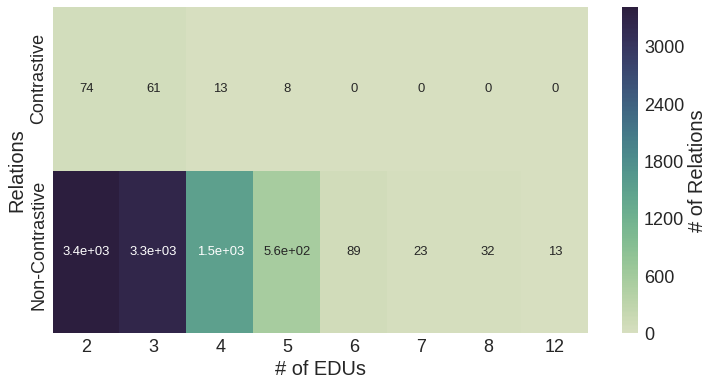
\includegraphics[width=\linewidth]{img/dasa_potts_rel_distribution.png}
      \caption{PotTS}\label{dasa:fig:relation-distribution-potts}
    \end{subfigure}
  }
  \centering
  {
    \centering
    \begin{subfigure}{0.7\textwidth}
      \centering
      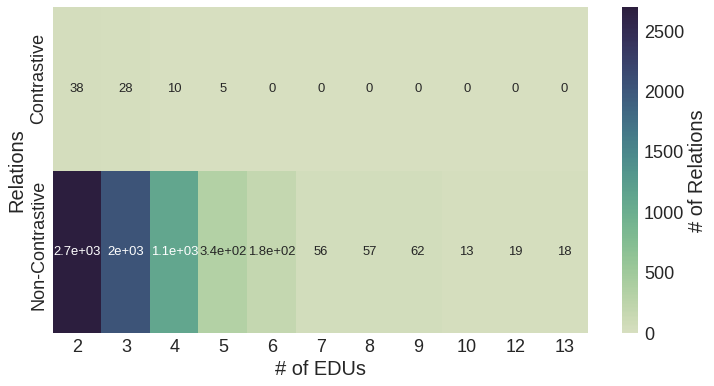
\includegraphics[width=\linewidth]{img/dasa_sb10k_rel_distribution.png}
      \caption{SB10k}\label{dasa:fig:relation-distribution-sb10k}
    \end{subfigure}
  }
  \caption[Relation distribution in PotTS and SB10k]{Distribution of
    Discourse Relations in the Training and Development Sets of PotTS
    and SB10k}\label{dasa:fig:relation-distribution}
\end{figure*}

\section{Discourse-Aware Sentiment Analysis}\label{sec:dasa:methods}

% \done[inline]{\citet{Bickerstaffe:10}}

% \citet{Bickerstaffe:10} also considered the rating prediction task,
% addressing this problem with the minimum-spanning-tree (MST) SVM
% approach.  In the initial step of this method, they constructed a
% strongly connected graph whose vertices were associated with the most
% representative example (determined via the average all-pairs Tanimoto
% coefficient) of each star rating and the edge weights represented the
% Tanimoto distances between those nodes.  Afterwards, they determined
% the MST of this graph using the Kruskal's
% algorithm~\cite[see][pp.~567--574]{Cormen:09} and, finally,
% constructed a decision tree from this MST, replacing the MST vertices
% with binary SVM classifiers, which had to discern the respective
% rating groups. An evaluation on the four-star review corpus
% of~\citet{Pang:05} showed an improvement by up to~7\% over the
% previous state of the art, boosting it to 59.37\% average accuracy.

Now, with these prepared data at hand, we are all set to check whether
incorporating the additional discourse information into our
lexicon-based attention system would improve the quality of its
analysis.  However, before we proceed with this check, let us first
revise the most prominent related approaches to discourse-aware
sentiment classification that have been proposed in the literature so
far.

As it turns out, even the very first works on opinion mining already
pointed out the importance of discourse phenomena for determining the
overall polarity of a text.  For example, in the seminal paper
of~\citet{Pang:02}, where the authors tried to predict the semantic
orientation of movie reviews, they quickly noticed the fact that it
was insufficient to rely on the mere presence or even majority of
polarity clues because these clues could any time be reversed by a
single counter-argument (see Example~\ref{disc-snt:exmp-pang02}).
\begin{example}[Polarity reversal via discourse antithesis]\label{disc-snt:exmp-pang02}
  \noindent\upshape This film should be brilliant.  It sounds like a
  great plot, the actors are first grade, and the supporting cast is
  good as well, and Stallone is attempting to deliver a good
  performance.  However, it can't hold up. \cite{Pang:02}
\end{example}
\noindent \citet{Polanyi:06} also affirmed the important role of the
text structure, considering discourse connectors and relations as one
of the most significant context factors which could notably affect the
intensity and polarity of opinions.  To prove this claim, they
provided several convincing examples in which concessive discourse
links considerably weakened the strength of a sentiment, and, vice
versa, increased the persuasiveness of a subjective argument by
elaborating.

These observations have rapidly motivated NLP researchers to add a
discourse-analysis component to document-level sentiment classifiers.
One of the first such systems was presented by~\citet{Pang:04}, who
tried to improve the classification accuracy on the IMDB corpus by
explicitly pointing the sentiment predictor to the sentences which
another (discourse-aware) classifier has previously considered as
subjective.  To achieve this goal (\ie{} to distinguish subjective
statements from objective), \citet{Pang:04} considered each text as a
graph whose vertices represented the sentences with their
automatically induced subjectivity scores (which were assigned
automatically by another classifer independently of the context) and
connected these vertices via affinity edges to their immediate
neighbors in text.  After adding two more abstract nodes which stood
for the subjective and objective classes and linking all sentences to
these two vertices, the authors determined the minimum cut of that
graph using the Blum algorithm \cite{Blum:01} and partitioned it into
two clusters (subjective and objective) on that cut.

Although an obvious oversimplification, the core idea that locally
adjacent sentences had to share the same subjective properties (local
coherence) has been dominating the following discourse-aware sentiment
research for almost a decade.  For example, \citet{Riloff:03} also
improved the accuracy of their Na{\"i}ve Bayes predictor of subjective
expressions by $\approx2\%$ after adding a set of discourse-related
coherence features.  Similarly, \citet{Hu:04} achieved better scores
on disambiguating users' polarities towards particular product
features after taking the information about the semantic orientation
of the previous sentences into account.

Another important line of DASA research concentrated more on the joint
analysis of opinions, where, in addition to classifying each sentiment
in isolation, the authors also sought to maximize the ``total
happiness'' (or global coherence) of these assignments by ensuring
that similar or related judgements recieved the same or at least
agreeing polarity scores.  One of the most notable works in this
direction was done by \citet{Snyder:07}, who introduced the Good Grief
algorithm for predicting the satisfaction of a user with different
aspects of a restaurant.  Another important contribution was made by
\citet{Somasundaran:08a,Somasundaran:08}, who proposed the concept of
\emph{opinion frames} (OF)---a special data structure for representing
the relations between the opinions in discourse.  Depending on the
type of these opinions (whether arguing~[\emph{A}] or
sentiment~[\emph{S}]), their polarity towards the target (whether
positive~[\emph{P}] or negative~[\emph{N}]), and the semantic
relationship between targets (whether alternative~[\emph{Alt}] or the
same~[\emph{same}]), the authors distinguished 32 types of possible
frames: \emph{SPSPsame}, \emph{SPSNsame}, \emph{APAPalt}, etc.,
dividing them into reinforcing and non-reinforcing ones.  Later on,
\citet{Somasundaran:09a,Somasundaran:09b} also presented two joint
inference frameworks (iterative classification and integer linear
programming) for determining the best configuration of all opinion
frames, achieving 77.72\% accuracy of frame prediction on the AMI
meeting corpus~\cite{Carletta:05}.

%% \done[inline]{\citet{Somasundaran:09a,Somasundaran:09b}}

%% In a later work, \citet{Somasundaran:09b,Somasundaran:09a} also
%% introduced a joint inference framework based on the Iterative
%% Classification Algorithm (ICA) and Integer Linear Programming (ILP)
%% for joinly predicting the best configuration of single opinions and
%% their frames.  In this approach, the authors first applied a local SVM
%% classifier to compute the probabilities of polarity classes (positive,
%% negative, or neutral) of individual dialog acts and then harnessed the
%% ICA and ILP systems to determine which of the predicted opinions were
%% connected via opinion frames and whether these frames were reinforcing
%% or not.  Given a perfect information about the opinion links, this
%% joint method outperformed the local classifier by more than 9
%% percentage points, reaching 77.72\% accuracy on the AMI meeting
%% corpus~\cite{Carletta:05}.

%% \done[inline]{\citet{Mao:06}}

%% \citet{Mao:06} proposed the idea of isotonic CRFs in which they
%% explicitly modeled the constraint that features which were stronger
%% associated with either polarity classes had to have higher
%% coefficients than less predictive attributes.  After proving that this
%% formalism also allowed to directly model the ordinal scale of
%% sentiment scores (with lower CRF outputs indicating the negativity of
%% a sentence, and higher scores showing its positive class), the authors
%% used this approach to model the sentiment flow in a document.  For
%% this purpose, they first predicted the polarity value for each
%% sentence of a document in isolation and then convolved these outputs
%% with a Gaussian kernel, getting a smoothed polarity curve for the
%% whole analyzed text at the end.
%% \done[inline]{\citet{Thomas:06}}

%% \citet{Thomas:06} enhanced an SVM-based sentiment classification
%% system for predicting speaker's attitude in political speeches with
%% information about the inter-speaker agreement, incorporating these
%% links into the global cost function.  Thanks to this change, the
%% authors achieved $\approx$4\% improvement in accuracy (from 66.05 to
%% 70.81\%) over the baseline classifer which analyzed each utterance in
%% isolation.

An attemt to reunite local and global coherence again was made by
\citet{McDonald:07}, who proposed a joint framework based on
\emph{latent variables} for simultaneously predicting the polarity of
a document and its constituent parts (which could be either paragraphs
or sentences).  For this purpose, the authors considered the semantic
orientation of the whole text and its single sentences as unobserved
variables in a Markov random field, connecting each such sentence node
to the vertices of its adjacent clauses and the overal polarity node
of the complete document, and then figuring out the best configuration
of all variables at the end.%%   A similar approach was also suggested
%% by~\citet{Sadamitsu:08}, who attained 82.74\% accuracy on predicting
%% the polarity of customer reviews with the help of hidden conditional
%% random fields.

Another latent-variable approach was presented by
\citet{Yessenalina:10}, who tried to predict the overall semantic
orientation of a document by first selecting a subset of the most
indicative sentences and then classifying the document (as either
positive or negative) with the help of this selection.  To achieve
this goal, the authors adopted the latent-SVM method of \citet{Yu:09}
by first training a linear classifier on individual sentences with
latent classes and then making the final prediction using 30\% of
those clauses which the classifier was most sure about.  With this
method, \citet{Yessenalina:10} attained 93.22\% accuracy on the movie
review corpus of \citet{Pang:04} and reached 77.09\% on a collection
of congressional floor debates \cite{Thomas:06}.

A common drawback of all these approaches though is their complete
ignoring of traditional discourse theories and, as a consequence of
this, too coarse approximation of discourse structure (which
essentially boils down to either connecting nearby sentences, or
creating a densely connected graph).  Among the first who tried to
overcome this omission were \citet{Voll:07}, who came up with two
different ways of making their lexicon-based sentiment calculator
\cite[SO-CAL; ][]{Taboada:11} aware of discourse information: In the
first method, they let the classifier analyze only the top-post
nucleus segment of each sentence (using automatically derived RST
trees for determining these EDUs).  In the second attempt, they
restricted the SO-CAL's input only to the clauses that had been
previously classified as pertaining to the main topic of the text.
Unfortunately, the RST-based solution did not work out as well as
expected and failed to outperform even the discourse-unaware baseline,
yielding only 69\% precision on a corpus of Epinion reviews
\cite{Taboada:06}.  This mishap, however, could be partially due to
the fact that the authors completely ignored all nuclei and satellites
apart from the roots and also disregarded all inter-sentential
relations.  The topic-aware method, however, turned out to work fairly
well, achieving 73\% accuracy on this two-class prediction task.

Other ways of incorporating discourse information into sentiment
systems were explored by \citet{Heerschop:11}, who experimented with
three different approaches:
\begin{inparaenum}[(i)]
\item increasing the polarity scores of words which appeared near
  the end of the document,
\item assigning higher weights to tokens in the nuclei of RST trees
  rather than satellites, and, finally,
\item training a genetic algorithm, which learned separate scores for
  the nuclei and satellite nodes.
\end{inparaenum}
An evaluation of these methods on the movie review corpus
of~\citet{Pang:04} showed a better performance of the first option
(0.608 accuracy and 0,597 macro-\F).  The authors, however, could
significantly improve the results of the last classifier at the end,
after adding an offset to the decision boundary, which increased both
its accuracy and macro~\F-measure to 0.72.

Other notable works on RST-based sentiment prediction were done by
\citet{Zhou:11}, who used a set of heuristic rules to infer possible
polarity shifts of discourse units based on their nuclearity status
and parent links, which allowed them to attain a statistically
significant improvement in sentence-level polarity classification on
the NTCIR MOAT corpus~\cite{Xu:10}; \citet{Zirn:11}, who applied a
lexicon-based sentiment system to compute the polarity scores of
elementary discourse units, and then enforced the consistency of these
assignments over an automatically derived RST tree with the help of of
Markov logic contraints; and, finally, \citet{Wang:13}, who also first
computed polarity scores of isolated discourse units and then
estimated the polarity of the whole document by taking a linear
combination of these scores, multiplying them with automatically
learned coefficients.\footnote{Similarly to the approach
  of~\citet{Zirn:11}, these coefficients depended on the status of the
  segment in the RST tree (whether nucleus or sattelite) and relation,
  which connected the respective discourse node to the ancestor.}  %% A
%% similar system was also described by \citet{Chenlo:13,Chenlo:14}, who
%% used their model to analyze user blog posts, achieving significantly
%% better results on the TREC corpus \cite{Macdonald:09} than any
%% discourse-unaware baselines.

Among the most recent advances in RST-based opinion mining, we should
especially emphasize the work of \citet{Bhatia:15}, who proposed two
different sentiment analysis systems:
\begin{itemize}
\item discourse depth reweighting (DDR)
\item and rhetorical recursive neural network (R2N2).
\end{itemize}
In the former approach, they estimated the relevance $\lambda_i$ of
each elementary discourse unit $i$ as:
\begin{equation*}
  \lambda_i = \max\left(0.5, 1 - d_i/6\right),
\end{equation*}
where $d_i$ stands for the depth of the $i$-th EDU in the document's
discourse tree; and computed the sentiment score $\sigma_i$ of that
unit as the dot product of its binary feature vector $\mathbf{w}_i$
(token unigrams) with the polarities of these features $\theta$ taken
from a lexicon:
\begin{equation*}
  \sigma_i = \theta^{\top}\cdot\mathbf{w}_i,
\end{equation*}
Afterwards, the authors calculated the overall semantic orientation of
the document~$\Psi$ as the sum of the predicted sentiment scores for
all units, multiplying these weights by the importance
factors~$\lambda$:
\begin{equation*}
  \Psi = \sum_i\lambda_i\mathbf{\theta}^T\mathbf{w}_i = \mathbf{\theta}^T\cdot\sum_i\lambda_i\mathbf{w}_i,
\end{equation*}

In the R2N2 method, \citet{Bhatia:15} adopted the RNN approach
of~\citet{Socher:13} by recursively computing the polarity score of
each discourse unit $i$ as:
\begin{equation*}
  \psi_i = tanh\left(K_n^{(r_i)} \psi_{n(i)} + K_s^{(r_i)}\psi_{s(i)} \right),
\end{equation*}
where $K_n^{(r_i)}$ and $K_s^{(r_i)}$ denote the nucleus and satellite
coefficients associated with the rhetorical relation $r_i$, whereas
$\psi_{n(i)}$ and $\psi_{s(i)}$ represent the sentiment scores of the
respective nodes.  This system achieved formidable 84.1\% two-class
prediction accuracy on the moview review corpus of~\citet{Pang:04} and
reached 85.6\% on the dataset of~\citet{Socher:13}.

For the sake of completeness, we should note that there also exist
discourse-aware sentiment approaches which build upon PDTB and SDRT:
For example, \citet{Trivedi:13} presented a method based on the latent
structural SVM~\cite{Yu:09}, in which they represented each sentence
as a vector of features produced by function $\mathbf{f}(y,
\mathbf{x}_i, h_i)$, where $y\in\{-1, +1\}$ denotes the potential
polarity of the document, $h_i \in \{0, 1\}$ represents the assumed
subjectivity class of sentence $i$, and $\mathbf{x}_i$ stands for the
surface form of the $i$-th sentence.  One such feature, for example,
could be \texttt{<+1, ``love'', 1>}, which would indicate that the
token ``love'' appears in a supposedly subjective sentence of a
positive document. However, because the true assignment of the
variables $h_i$ was unknown, the authors regarded this value as a
latent variable and tried to predict the most likely semantic
orientation of the document $\hat{y}$ by finding the maximum product
of weight and feature vectors over all possible assignments of
$\mathbf{h}$, \ie{}:
\begin{equation*}
  \hat{y} =
  \argmax_y\left(\max_{\mathbf{h}}\mathbf{w}^{\top}\mathbf{f}(y,
  \mathbf{x}, \mathbf{h})\right).
\end{equation*}
However, to ensure that these assignments were still coherent, the
authors additionally extended their original feature set with special
\emph{transitional} attributes, which indicated whether two adjacent
sentences were likely to share the same subjectivity given the
discourse connective between them.  With the help of these features,
they could improve the prediction accuracy on the movie review corpus
of~\citet{Maas:11} from 88.21 to 91.36\% in comparison with the
connector-unaware model.

The first steps towards an SDRT-inspired approach were made by
\citet{Asher:08}, who presented an annotation scheme and pilot corpus
of English and French texts labeled with their discourse structure
according to the SDRT theory and augmented with an additional
sentiment layer.  In particular, the authors asked the annotators to
ascribe one of four opinion categories (reporting, judgement, advice,
or sentiment) along with their subcategories (e.g., inform, assert,
blame, recommend) to each discourse unit which featured at least one
opinionated word from a sentiment lexicon.  Afterwards, they showed
that with a simple set of rules, one could easily propagate opinions
through the discourse graphs, increasing their strengths or reversing
their polarity, depending on the type of discourse relations that
connected the segments.

In general, however, PDTB- and SDRT-based sentiment analysis methods
are much less common than RST-inspired techniques, and since the focus
of this chapter is mainly on RST, we will next present an evaluation
of the most common approaches from this paradigm on the PotTS and
SB10k data.  To this end, we have reimplemented the DDR and R2N2
systems of~\citet{Bhatia:15}

\begin{table}[h]
  \begin{center}
    \bgroup \setlength\tabcolsep{0.1\tabcolsep}\scriptsize
    \begin{tabular}{p{0.162\columnwidth} % first columm
        *{9}{>{\centering\arraybackslash}p{0.074\columnwidth}} % next nine columns
        *{2}{>{\centering\arraybackslash}p{0.068\columnwidth}}} % last two columns
      \toprule
      \multirow{2}*{\bfseries Method} & %
      \multicolumn{3}{c}{\bfseries Positive} & %
      \multicolumn{3}{c}{\bfseries Negative} & %
      \multicolumn{3}{c}{\bfseries Neutral} & %
      \multirow{2}{0.068\columnwidth}{\bfseries\centering Macro\newline \F{}} & %
      \multirow{2}{0.068\columnwidth}{\bfseries\centering Micro\newline \F{}}\\
      \cmidrule(lr){2-4}\cmidrule(lr){5-7}\cmidrule(lr){8-10}

      & Precision & Recall & \F{} & %
      Precision & Recall & \F{} & %
      Precision & Recall & \F{} & & \\\midrule

      \multicolumn{12}{c}{\cellcolor{cellcolor}PotTS}\\

      %% General Statistics:
      HCRF & \textbf{0.76} & 0.79 & \textbf{0.77} & %
      0.61 & 0.53 & 0.57 & %
      0.7 & 0.71 & 0.7 & %
      0.67 & 0.708\\

      %% General Statistics:
      HMCRF & \textbf{0.76} & 0.79 & \textbf{0.77} & %
      \textbf{0.63} & 0.49 & 0.55 & %
      0.69 & \textbf{0.75} & \textbf{0.72} & %
      0.662 & \textbf{0.713}\\

      %% General Statistics:
      RDP & 0.71 & \textbf{0.83} & \textbf{0.77} & %
      0.59 & 0.55 & 0.57 & %
      \textbf{0.73} & 0.61 & 0.66 & %
      0.667 & 0.693\\

      %% General Statistics:
      WNG & 0.58 & 0.79 & 0.67 & %
      0.61 & 0.21 & 0.31 & %
      0.61 & 0.57 & 0.59 & %
      0.487 & 0.59\\

      %% General Statistics:
      DDR & 0.73 & 0.77 & 0.75 & %
      0.54 & \textbf{0.59} & 0.56 & %
      0.69 & 0.61 & 0.65 & %
      0.655 & 0.674\\

      %% General Statistics:
      R2N2 & 0.74 & 0.78 & 0.76 & %
      0.59 & 0.53 & 0.56 & %
      0.68 & 0.68 & 0.68 & %
      0.657 & 0.692\\

      %% General Statistics:
      \textsc{Last} & 0.52 & 0.83 & 0.64 & %
      0.57 & 0.17 & 0.26 & %
      0.61 & 0.43 & 0.5 & %
      0.453 & 0.549\\

      %% General Statistics:
      \textsc{Root} & 0.56 & 0.73 & 0.64 & %
      0.58 & 0.22 & 0.32 & %
      0.55 & 0.54 & 0.54 & %
      0.481 & 0.56\\

      %% General Statistics:
      \textsc{No-Discourse} & 0.73 & 0.82 & \textbf{0.77} & %
      0.61 & 0.56 & \textbf{0.58} & %
      0.72 & 0.66 & 0.69 & %
      \textbf{0.677} & 0.706\\

      \multicolumn{12}{c}{\cellcolor{cellcolor}SB10k}\\

      %% General Statistics:
      HCRF & \textbf{0.64} & \textbf{0.69} & 0.66 & %
      0.45 & \textbf{0.45} & 0.45 & %
      \textbf{0.82} & 0.79 & \textbf{0.8} & %
      0.557 & 0.713\\

      %% General Statistics:
      HMCRF & \textbf{0.64} & \textbf{0.69} & 0.66 & %
      0.44 & \textbf{0.45} & 0.45 & %
      \textbf{0.82} & 0.79 & \textbf{0.8} & %
      0.556 & 0.712\\

      %% General Statistics:
      RDP & \textbf{0.64} & \textbf{0.69} & \textbf{0.67} & %
      0.45 & \textbf{0.45} & 0.45 & %
      \textbf{0.82} & 0.79 & \textbf{0.8} & %
      \textbf{0.559} & \textbf{0.715}\\

      WNG & 0.61 & 0.63 & 0.62 & %
      0.46 & 0.29 & 0.36 & %
      0.76 & \textbf{0.82} & 0.79 & %
      0.488 & 0.693\\

      %% General Statistics:
      DDR & 0.59 & 0.63 & 0.61 & %
      \textbf{0.48} & 0.44 & \textbf{0.46} & %
      0.77 & 0.76 & 0.77 & %
      0.534 & 0.681\\

      %% General Statistics:
      R2N2 & \textbf{0.64} & \textbf{0.69} & 0.66 & %
      0.46 & \textbf{0.45} & 0.45 & %
      0.81 & 0.79 & \textbf{0.8} & %
      \textbf{0.559} & 0.713\\

      %% General Statistics:
      \textsc{Last} & 0.56 & 0.55 & 0.56 & %
      0.46 & 0.29 & 0.36 & %
      0.73 & 0.8 & 0.76 & %
      0.459 & 0.661\\

      %% General Statistics:
      \textsc{Root} & 0.51 & 0.55 & 0.53 & %
      0.4 & 0.3 & 0.35 & %
      0.74 & 0.76 & 0.75 & %
      0.438 & 0.64\\

      %% General Statistics:
      \textsc{No-Discourse} & \textbf{0.64} & \textbf{0.69} & 0.66 & %
      0.45 & \textbf{0.45} & 0.45 & %
      \textbf{0.82} & 0.79 & \textbf{0.8} & %
      0.557 & 0.713\\\bottomrule
    \end{tabular}
    \egroup
    \caption[Evaluation of DASA methods]{Evaluation of discourse-aware
      sentiment analysis methods\\ {\small HCRF~--~hidden conditional random fields,
        HMCRF~--~hidden marginalized conditional random fields,
        RDP~--~recursive Dirichlet process,
        WNG~--~\citet{Wang:13},
        DDR~--~discourse-depth reweighting~\cite{Bhatia:15},
        R2N2~--~rhetorical recursive neural network~\cite{Bhatia:15},
        \textsc{Last}~--~polarity determined by the last EDU,
        \textsc{Root}~--~polarity determined by the root EDU(s),
        \textsc{No-Discourse}~--~discourse-unaware classifier}}
    \label{dasa:tbl:res}
  \end{center}
\end{table}

\section{Evaluation}

\subsection{Base Classifier}

\subsection{Parsing Quality}

\subsection{Relation Scheme}

\begin{table}[h]
  \begin{center}
    \bgroup \setlength\tabcolsep{0.1\tabcolsep}\scriptsize
    \begin{tabular}{p{0.17\columnwidth} % first columm
        *{1}{>{\centering\arraybackslash}p{0.4\columnwidth}}
        *{1}{>{}p{0.4\columnwidth}}} % next two columns
      \toprule
      \textbf{Scheme} & \textbf{Relation Set} & \textbf{Equivalence Classes}\\\midrule

      \textsc{PCC} & \{ \textsc{Antithesis}, \textsc{Background},
      \textsc{Cause}, \textsc{Circumstance}, \textsc{Concession},
      \textsc{Condition}, \textsc{Conjunction}, \textsc{Contrast},
      \textsc{Disjunction}, \textsc{E-Elaboration},
      \textsc{Elaboration}, \textsc{Enablement},
      \textsc{Evaluation-N}, \textsc{Evaluation-S}, \textsc{Evidence},
      \textsc{Interpretation}, \textsc{Joint}, \textsc{Justify},
      \textsc{List}, \textsc{Means}, \textsc{Motivation},
      \textsc{Otherwise}, \textsc{Preparation}, \textsc{Purpose},
      \textsc{Reason}, \textsc{Restatement}, \textsc{Restatement-MN},
      \textsc{Result}, \textsc{Sequence}, \textsc{Solutionhood},
      \textsc{Summary}, \textsc{Unconditional}, \textsc{Unless},
      \textsc{Unstated-Relation}\} & \\

      \citet{Heerschop:11} & \{\textsc{Attribution},
      \textsc{Background}, \textsc{Cause}, \textsc{Condition},
      \textsc{Contrast}, \textsc{Elaboration}, \textsc{Enablement},
      \textsc{Explanation}, \textsc{\bfseries Other}\} & \\

      \citet{Zhou:11} & \{\textsc{Contrast}, \textsc{Condition},
      \textsc{Continuation}, \textsc{Cause}, \textsc{Purpose},
      \textsc{\bfseries Other}\} & \textsc{Contrast} $\defeq$
      \{\textsc{Antithesis}, \textsc{Concession}, \textsc{Otherwise},
      \textsc{Contrast}\};\newline \textsc{Continuation} $\defeq$
      \{\textsc{Continuation}, \textsc{Parallel}\};\newline
      \textsc{Cause} $\defeq$ \{\textsc{Evidence}, \textsc{Volitional
        Cause}, \textsc{Nonvolitional-Cause},
      \textsc{Volitional-Result}, \textsc{Nonvolitional-Result}\};\\

      \citet{Chenlo:13} & \{\textsc{Attribution}, \textsc{Background},
      \textsc{Cause}, \textsc{Comparison}, \textsc{Condition},
      \textsc{Consequence}, \textsc{Contrast}, \textsc{Elaboration},
      \textsc{Enablement}, \textsc{Evaluation}, "Explanation",
      \textsc{Joint}, \textsc{Otherwise}, \textsc{Temporal},
      \textsc{\bfseries Other}\} & \\

      \citet{Bhatia:15} & \{\textsc{Contrastive},
      \textsc{\bfseries Non-Contrastive}\} & \textsc{Contrastive} $\defeq$
      \{\textsc{Antithesis}, \textsc{Antithesis-E},
      \textsc{Comparison}, \textsc{Concession},
      \textsc{Consequence-S}, \textsc{Contrast},
      \textsc{Problem-Solution}\}.\\\bottomrule
\end{tabular}
    \egroup
    \caption[RST relations used in different discourse-aware sentiment
      methods]{RST relations used in the original Potsdam Commentary
      Corpus and different discourse-aware sentiment methods\\ {\small
        (default relation [which subsumes the rest of the links] is
        highlighted in \textbf{boldface})}}
    \label{dasa:tbl:rst-rels}
  \end{center}
\end{table}

\begin{table}[h]
  \begin{center}
    \bgroup \setlength\tabcolsep{0.1\tabcolsep}\scriptsize
    \begin{tabular}{p{0.22\columnwidth} % first columm
        *{3}{>{\centering\arraybackslash}p{0.25\columnwidth}}} \toprule

      \textbf{Relation Scheme} & \textbf{Span \F{}} &
       \textbf{Nuclearity \F{}} & \textbf{Relation \F{}}\\\midrule

      \textsc{PCC} & 0.776 & 0.534 & 0.326\\

      \citet{Heerschop:11} & 0.774 & 0.51 & 0.361\\

      \citet{Zhou:11} & 0.776 & 0.501 & 0.388\\

      \citet{Chenlo:13} & 0.769 & 0.505 & 0.362\\

      \citet{Bhatia:15} & 0.777 & 0.512 & 0.396\\\bottomrule
\end{tabular}
    \egroup
    \caption[Results of RST parser on PCC~2]{Results of automatic RST
      parser on PCC~2.0 with different relation schemes}
    \label{dasa:tbl:rst-rels}
  \end{center}
\end{table}

\section{Summary and Conclusions}
